In this work, we investigate the utility of Recurrent Neural Networks (\textsc{rnn}s) for script and langauge identification. Both these problems have been attempted in the past with representations computed from the distribution of connected components or characters (e.g. texture, $n$-gram). Often these features are computed from a larger segment (a paragraph or a page). We argue that one can predict the script or language with minimal evidence
(e.g. given only a word or a line) very accurately with the help of a pre-trained \textsc{rnn}. %Our solution
%is simple and accurate even without any special tuning for the scripts or language of interest.
We propose a simple and generic solution for the task of script and language identification which do not require any special tuning.
%We propose a simple and accurate solution independent of special tuning for the scripts or language of interest.
Our method represents the word images as a sequence of feature vectors, and employ the \textsc{rnn}s for the identification. We verify the method on a large corpus of more than 15.03M words from 55K document images comprising 15 scripts and languages. We report an accurate script and language identification at word and line level.
%We also comment on some of the future directions for such recognition-free solutions.
%\end{abstract}
%
%\begin{keywords}
%Script and Language Identification, Recurrent Neural Networks, Recognition Free Methods
%\end{keywords}

\section{Introduction}
\label{sec:intro}

Recurrent Neural Networks (\textsc{rnn}s) have gained popularity in recent years for many recognition tasks such as Optical Character Recognition(\textsc{ocr})~\cite{Breuel13,PraveenDAS}, handwriting recognition{~\cite{GravesLFBBS09}}, word retrieval{~\cite{Volkmar11}}, and word spotting~\cite{Manmatha12}. This architecture has started finding more and more applications in diverse areas of computer vision~\cite{Hinton12}. In this work, we investigate the utility of \textsc{rnn}s for script and language identification at the granularity of words
and lines. Naturally, this investigation has its applications in multilingual settings, where one 
needs to decide the script or language before recognition or post-processing of an incoming document image. In addition, this work also throws light on how semantically richer tasks can be attempted without any explicit recognition by looking at the distribution of certain features. For example, can we find the topic model or classify the document into an appropriate category without an explicit textual representation? Such high-level tasks are often attempted based on the statistics and distribution of words or characters. In this work, we limit our attention to the identification of script and language at the word and line level as shown in Fig.~\ref{fig:demoResults}. By designing an \textsc{rnn} that can learn the distribution of feature vectors, we reliably identify the scripts and language from the image itself. We empirically demonstrate the utility of \textsc{rnn}s for script and language identification with experiments on a corpus of nearly 15.03M words from 55K document images comprising 15 scripts and languages. We argue that \textsc{rnn}s can be considered as a strong contender for accurate script and language identification which can lead us to the integrated solutions for the recognition tasks in multilingual settings.

\begin{figure}[t]
\begin{center}
%\fbox{
\tabcolsep=0.20cm
\def\arraystretch{0.5}
\begin{tabular}{cc}
{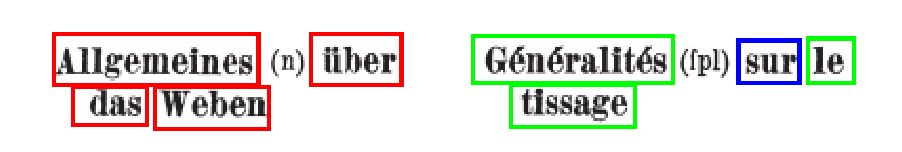
\includegraphics[scale=0.545]{/home/ajeet/Dropbox/Singh_ICDAR15/images/red_hot_1.eps}} \\
{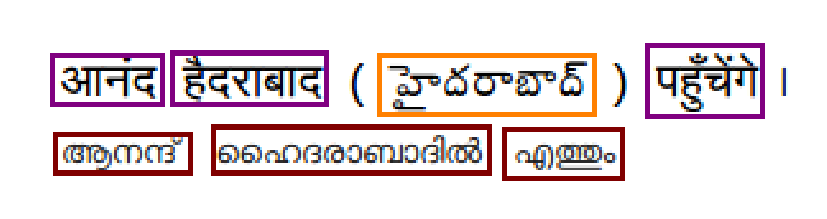
\includegraphics[scale=0.6]{/home/ajeet/Dropbox/Singh_ICDAR15/images/script_pic_1.eps}}
\\
\end{tabular}
%}
\end{center}
\caption{Figure depicts the script and language identified at word level in document snippets written in Roman-script (first row) based languages and Indic scripts (second row), respectively. In the first row, red, green and blue rectangles denote German, French and Spanish languages, respectively. In the second row, violet, orange and brown rectangles denote Hindi, Telugu and Malayalam scripts, respectively. Unlike the approaches in the past we propose a method to identify the script and language at word and line level by employing popular Recurrent Neural Network (\textsc{rnn}s).}
\label{fig:demoResults}
\end{figure}

%\begin{figure}
%\begin{minipage}[c][3cm][t]{.48\textwidth}
%  \vspace*{\fill}
%  \centering
%  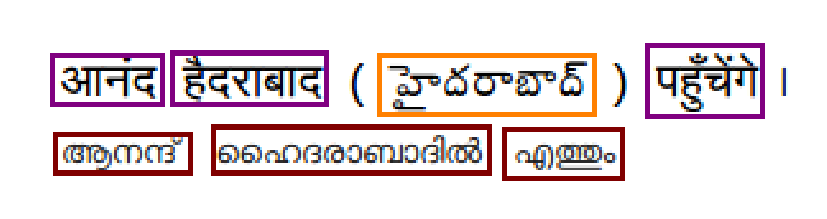
\includegraphics[scale=0.60]{/home/ajeet/Dropbox/Singh_ICDAR15/images/script_pic_1.eps}
%  %\caption{test figure two}
% \label{fig:test2}\par\vfill
% 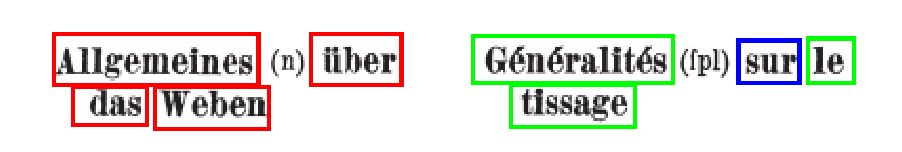
\includegraphics[scale=0.545]{/home/ajeet/Dropbox/Singh_ICDAR15/images/red_hot_1.eps}
%  %\caption{test figure three}
%\label{fig:test3}
%\end{minipage}
%\caption{Figure depicts the script and language identified at word level in document snippets written in Indic scripts(first row) and Roman-script(second row) based languages, respectively. In first row, violet, orange and brown rectangles denote Hindi, Telugu and Malayalam scripts, respectively. In second row, red, green and blue rectangles denote German, French and Spanish languages, respectively. Unlike the approaches in the past we propose a method to identify the script and language at word and line level by employing popular Recurrent Neural Network (\textsc{rnn}s).}
%\label{fig:demoResults}
%\end{figure}

Many approaches proposed in the past for script and language identification often deal at page, line or word level. At page level, script is identified by looking at the texture and orientation of the image segments. Sptiz~\cite{Spitz97} analylzed the individual components for script identification in document images using attributes such as upward concavities, optical densities, character height densities and top and bottom profiles. The use of texture has also been extensively used in script identification. Tan~\cite{Tan98} proposed to solve this problem using a multi-channel Gabor filter. Many later attempts used different variations of texture features computed from Gray-level Co-occurrence Matrix, Gabor Energy, Wavelet Energy, Local Binary Pattern~\cite{Busch05,Ferrer13,Pati,sukalpa09} for the identification purpose. In recent years, there has been an effort to use discriminative features learned using Convolutional Neural Networks(\textsc{CNN}) for multi-script recognition~\cite{Rashid10}. These features are automatically extracted and learned at connected component level of the document image. % Most of these works were motivated by the need of building a multilingual \textsc{ocr}. There has also been some motivating arguments to support the document image analysis needs of multilingual countries like India.

When the inherent script of document images are same, visual features are hard to separate between different languages, especially when the identification is required at word level. There are many attempts in the textual domain to separate the languages. Often they use the statistics (\eg\ $n$-gram probabilities of characters). In the image domain, language identification is attempted at page level or paragraph level in the past.
A class of methods have been proposed which categorizes the characters based on a number of character shape features such as character ascenders and descenders. For example,~\cite{Spitz97} group the character images into a small set of categories first. Then, based on the classification results, each word image is converted into a word shape token. Latin-based languages are finally determined according to the frequency of a single word~\cite{Spitz97}, word pair and word trigram. Shijian and Tan~\cite{Shijian08}
combined the script and language identification using a document vectorization framework. They convert document image into a vertical cut vector based on the number and positions of vertical cut to capture the shape of the word directly.

%Many approaches in the past for script and language identification often deal at page, line or word level. At page level, script is often separated at by looking at the texture and orientation of the image segments.
%Spitz~\cite{Spitz97} analyzed the individual components for script identification in document images using attributes such as upward concavities, optical densities, character height densities, top and bottom profiles. The use of texture has also been extensively used in script identification. Tan~\cite{Tan98} proposed to solve this problem using a multi-channel Gabor filter. Many later attempts used different variations of texture features computed from Gray-level Co-occurrence Matrix, Gabor Energy, Wavelet Energy, Local Binary Pattern~\cite{Busch05,Ferrer13,Pati,sukalpa09}. Most of these works were motivated by the need of building a multilingual \textsc{ocr}. There has also been motivating arguments to support the document 
%image analysis needs of multilingual countries like India. When the scripts are same, visual features are hard to separate between languages, especially when the identification required are at word level. There are many attempts in the textual domain to separate the languages. Often they use the statistics ($n$-grams probabilities of characters). In the image domain, language identification is attempted at page level or paragraph level in the past.
%A class of methods in the past categorizes the characters based on a number of character shape features such as character ascenders and descenders. For e.g.~\cite{Spitz97} group the character images into a small set of categories first. Then, based on the classification results, each word image is converted into a word shape token. Latin-based languages are finally determined according to the frequency of a single word~\cite{Spitz97}, word pair and word trigram. Shijian \emph{et al.}~\cite{Shijian08}
%combine the script and language identification using a document vectorization framework which converts document image into a vertical cut vector based on the number and positions of vertical cut which then captures the shape of the word directly. In recent years, there have been an effort to use discriminative features learned using Convolutional Neural Networks(\textsc{CNN}) for multi-script recognition~\cite{Rashid10}. These features are automatically extracted and learned at connected component level of document image.

Our method is simple, efficient and accurate, without any special tuning for the scripts or languages of interest. We convert the word or line images into a sequence of feature vectors and train the \textsc{rnn}s to reliably separate the script or language.  We report comparable, if not better results than the state-of-the-art~\cite{Pati}. Our method also leaves lots of scope for further improvement in performance with better features and special adjustments (e.g. hierarchical classification, special features for harder pairs). We believe this makes our method very generic and applicable in a wide range of settings. We perform the experiments on 12 Indic scripts: Hindi, Malayalam, Gurumukhi, Kannada, Tamil, Telugu, Bangla, Marathi, Gujarati, Assamese, Manipuri and Odiya, and 3 Roman script based languages: French, German and Spanish (Figure.~\ref{fig:exImgs}).  We discuss the method in Section~\ref{sec:scriptLangId} and the experimental results in Section~\ref{sec:experiments}.

\begin{table}[h]
\centering
\renewcommand{\arraystretch}{1.5}
\begin{tabular}{|l|c|c|c|c|}
\hline
\textbf{Languages} & \multicolumn{4}{c|}{\textbf{Images}} \\ \hline\hline
Hindi & 
\includegraphics[width=1.65cm,height=0.35cm]{figures/hindi_right_1.eps} & 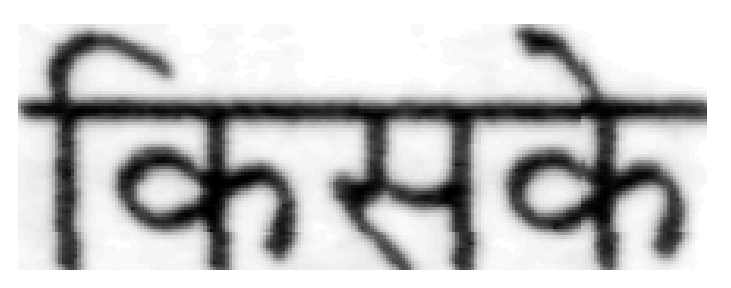
\includegraphics[width=1.65cm,height=0.35cm]{figures/hindi_right_2.eps} &  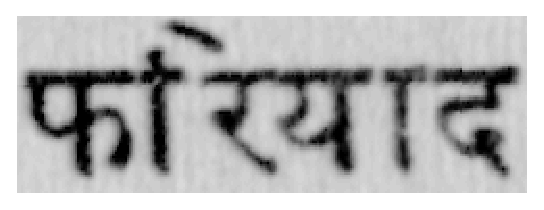
\includegraphics[width=1.65cm,height=0.35cm]{figures/hindi_right_3.eps}  & 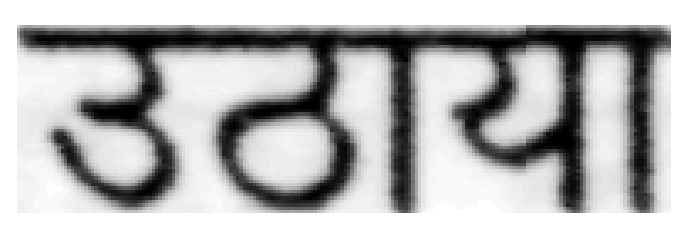
\includegraphics[width=1.65cm,height=0.35cm]{figures/hindi_right_4.eps} \\ \hline
Malayalam & 
\includegraphics[width=1.65cm,height=0.35cm]{figures/malayalam_right_3.eps} & 
\includegraphics[width=1.65cm,height=0.35cm]{figures/malayalam_right_2.eps} &  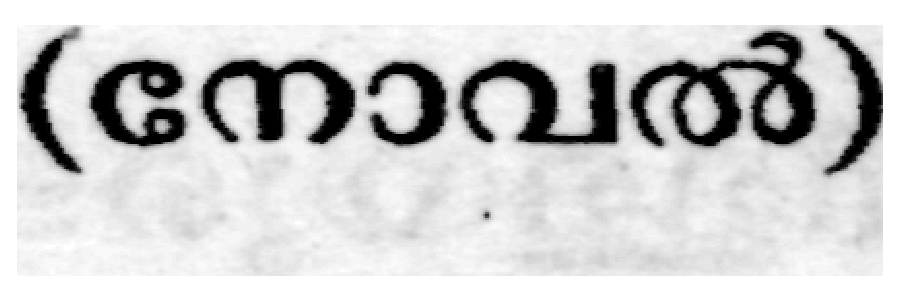
\includegraphics[width=1.65cm,height=0.35cm]{figures/malayalam_right_1.eps}  & 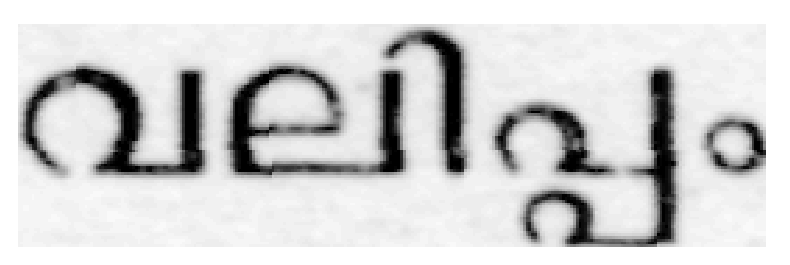
\includegraphics[width=1.65cm,height=0.35cm]{figures/malayalam_right_4.eps} \\ \hline
Gurumukhi &  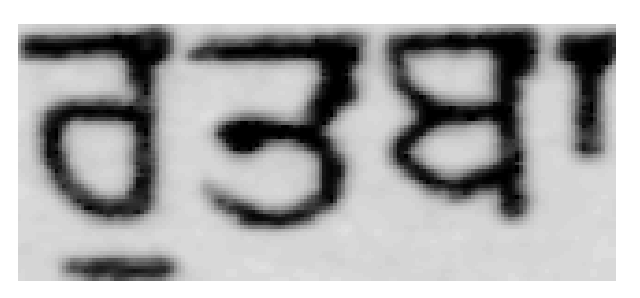
\includegraphics[width=1.65cm,height=0.35cm]{figures/gurumukhi_right_2.eps} & 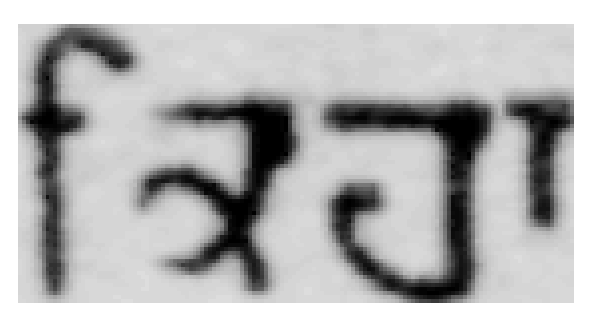
\includegraphics[width=1.65cm,height=0.35cm]{figures/gurumukhi_right_3.eps} &  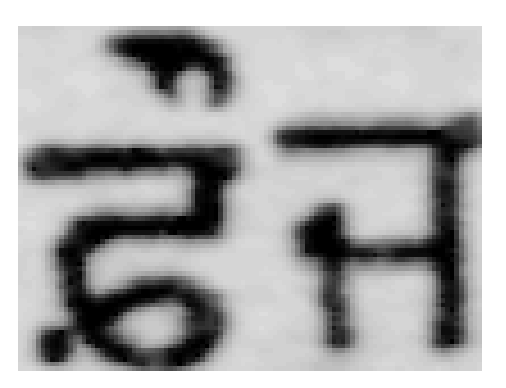
\includegraphics[width=1.65cm,height=0.35cm]{figures/gurumukhi_right_1.eps}  & 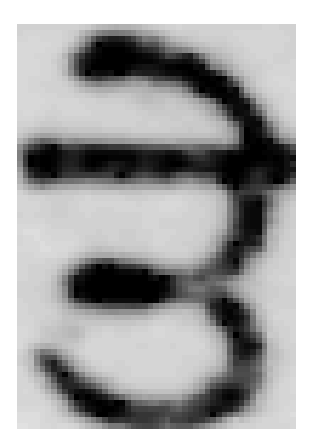
\includegraphics[width=1.65cm,height=0.35cm]{figures/gurumukhi_right_4.eps} \\ \hline
Kannada & 
\includegraphics[width=1.65cm,height=0.35cm]{figures/kannada_right_1.eps}  & 
\includegraphics[width=1.65cm,height=0.35cm]{figures/kannada_right_2.eps} &  
\includegraphics[width=1.65cm,height=0.35cm]{figures/kannada_right_3.eps}  & 
\includegraphics[width=1.65cm,height=0.35cm]{figures/kannada_right_4.eps}  \\ \hline
Tamil & 
\includegraphics[width=1.65cm,height=0.35cm]{figures/tamil_right_1.eps}  & 
\includegraphics[width=1.65cm,height=0.35cm]{figures/tamil_right_2.eps} &  
\includegraphics[width=1.65cm,height=0.35cm]{figures/tamil_right_3.eps}  & 
\includegraphics[width=1.65cm,height=0.35cm]{figures/tamil_right_4.eps} \\ \hline
Telugu & 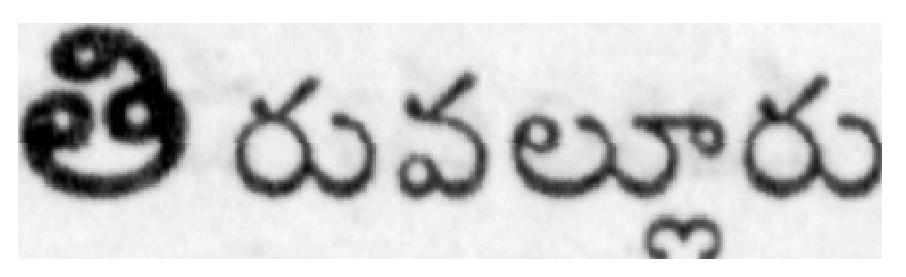
\includegraphics[width=1.65cm,height=0.35cm]{figures/telugu_right_1.eps}  & 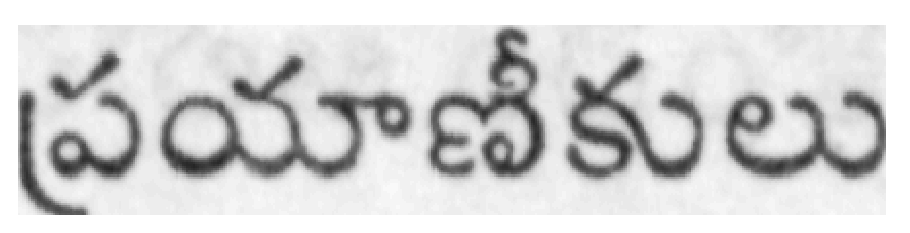
\includegraphics[width=1.65cm,height=0.35cm]{figures/telugu_right_2.eps} &  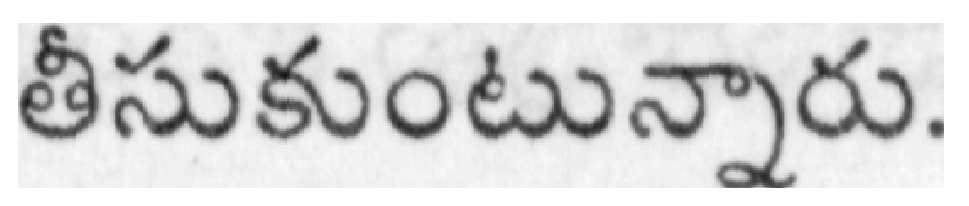
\includegraphics[width=1.65cm,height=0.35cm]{figures/telugu_right_3.eps}  & 
\includegraphics[width=1.65cm,height=0.35cm]{figures/telugu_right_4.eps} \\ \hline
Bangla & 
\includegraphics[width=1.65cm,height=0.35cm]{figures/bangla_right_1.eps}  & 
\includegraphics[width=1.65cm,height=0.35cm]{figures/bangla_right_2.eps} &  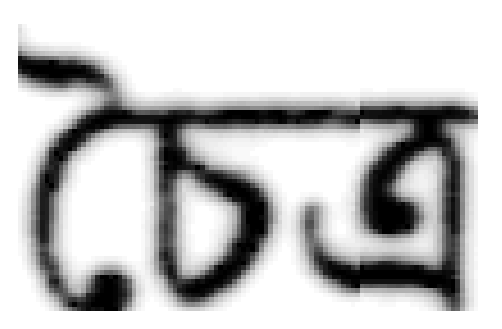
\includegraphics[width=1.65cm,height=0.35cm]{figures/bangla_right_3.eps}  & 
\includegraphics[width=1.65cm,height=0.35cm]{figures/bangla_right_4.eps} \\ \hline
Marathi & 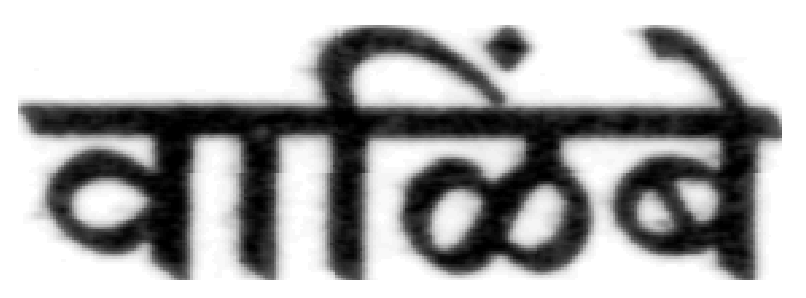
\includegraphics[width=1.65cm,height=0.35cm]{figures/marathi_right_1.eps}  & 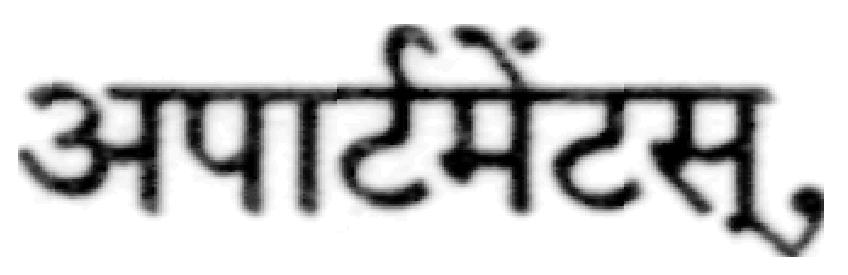
\includegraphics[width=1.65cm,height=0.35cm]{figures/marathi_right_2.eps} &  
\includegraphics[width=1.65cm,height=0.35cm]{figures/marathi_right_3.eps}  & 
\includegraphics[width=1.65cm,height=0.35cm]{figures/marathi_right_4.eps}  \\ \hline
Gujarati & 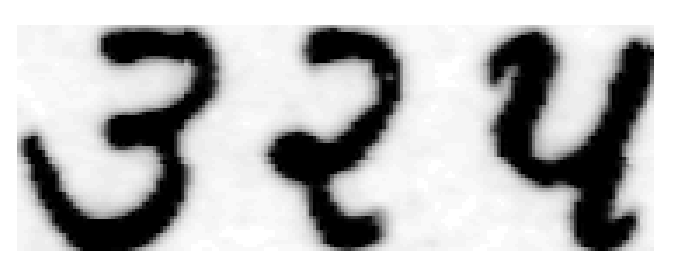
\includegraphics[width=1.65cm,height=0.35cm]{figures/gujrathi_right_1.eps}  & 
\includegraphics[width=1.65cm,height=0.35cm]{figures/gujrathi_right_2.eps} &  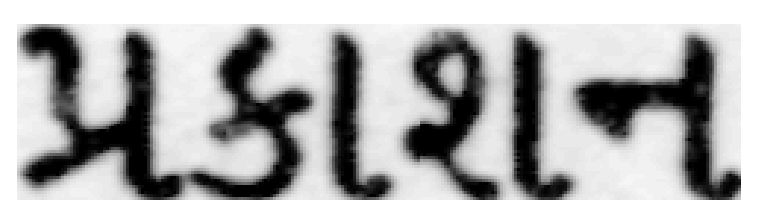
\includegraphics[width=1.65cm,height=0.35cm]{figures/gujrathi_right_3.eps}  & \includegraphics[width=1.65cm,height=0.35cm]{figures/gujrathi_right_4.eps}  \\ \hline
Assamese & 
\includegraphics[width=1.65cm,height=0.35cm]{figures/assamese_right_1.eps}  & 
\includegraphics[width=1.65cm,height=0.35cm]{figures/assamese_right_2.eps} &  
\includegraphics[width=1.65cm,height=0.35cm]{figures/assamese_right_3.eps}  & 
\includegraphics[width=1.65cm,height=0.35cm]{figures/assamese_right_4.eps}  \\ \hline
Manipuri &  
\includegraphics[width=1.65cm,height=0.35cm]{figures/manipuri_right_1.eps}  & 
\includegraphics[width=1.65cm,height=0.35cm]{figures/manipuri_right_2.eps} &  
\includegraphics[width=1.65cm,height=0.35cm]{figures/manipuri_right_3.eps}  & 
\includegraphics[width=1.65cm,height=0.35cm]{figures/manipuri_right_4.eps}  \\ \hline
Oriya &  
\includegraphics[width=1.65cm,height=0.35cm]{figures/oriya_right_1.eps}  & 
\includegraphics[width=1.65cm,height=0.35cm]{figures/oriya_right_2.eps}  &  \includegraphics[width=1.65cm,height=0.35cm]{figures/oriya_right_3.eps}  & \includegraphics[width=1.65cm,height=0.35cm]{figures/oriya_right_4.eps}\\ \hline\hline
French & \includegraphics[width=1.65cm,height=0.35cm]{figures/french_right_1.eps}  & \includegraphics[width=1.65cm,height=0.35cm]{figures/french_right_2.eps} &  \includegraphics[width=1.65cm,height=0.35cm]{figures/french_right_3.eps}  & \includegraphics[width=1.65cm,height=0.35cm]{figures/french_right_4.eps} \\ \hline
German &  \includegraphics[width=1.65cm,height=0.35cm]{figures/german_right_1.eps}  & \includegraphics[width=1.65cm,height=0.35cm]{figures/german_right_2.eps} &  \includegraphics[width=1.65cm,height=0.35cm]{figures/german_right_3.eps}  & \includegraphics[width=1.65cm,height=0.35cm]{figures/german_right_4.eps} \\ \hline
Spanish &  \includegraphics[width=1.65cm,height=0.35cm]{figures/spanish_right_1.eps}  & \includegraphics[width=1.65cm,height=0.35cm]{figures/spanish_right_2.eps} &  \includegraphics[width=1.65cm,height=0.35cm]{figures/spanish_right_3.eps}  & \includegraphics[width=1.65cm,height=0.35cm]{figures/spanish_right_4.eps} \\ \hline
\end{tabular}
\caption{Some example images from 12 Indic Scripts and 3 Roman script based languages.}
\label{fig:exImgs}
\end{table}

%\newpage
\section{\textsc{rnn} for Script and Language Identification}
\label{sec:scriptLangId}
In traditional feed-forward neural networks (\textsc{ffnn}), connections between the nodes do not form any cycles. If we relax this condition, and allow the cyclical connections among the nodes, we obtain the \textit{recurrent neural networks} (\textsc{rnn}s). \textsc{rnn}s in the past have been used to handle sequential data. \textsc{rnn} is a powerful classification tool, as it allows a ``memory" regarding previous inputs to persist in network's internal state, which can be  later used to influence the network output. \textsc{rnn}s are not widely popular, as they often require a longer training process, because the error path integral decays exponentially along the sequence~\cite{Schmidhuber97}. Our preference for \textsc{rnn}s is motivated by the fact that it has superior characteristics in several aspects. %unlike its counterparts e.g. \textsc{svm}, \textsc{hmm}, or a traditional neural network. 
Unlike \textsc{hmm} which uses the current state of input to generate any observations, \textsc{rnn} uses the long-short term memory (\textsc{lstm}~\cite{GravesLFBBS09}) structure to store the contextual information of previous states. Also it does not require any explicit labeling of all the vectors in the input feature sequences.

For the script and language identification, we use a \textsc{rnn} based Bidirectional Long Short Term Memory(\textsc{blstm}) network. These networks have been used in the past for  printed text~\cite{PraveenDAS} and handwritten text recognition~\cite{GravesLFBBS09}. This network consists of two \textsc{lstm} networks in which one network takes the input from beginning to end while other network takes the input from end to beginning. The individual output of both the \textsc{lstm} networks is used to predict the final output. Hence, these networks have been known for remembering the long range of context over several timesteps. The Connectionist Temporal Classification (\textsc{ctc})~\cite{GravesFGS06} is used at the output layer of \textsc{rnn} network to label the unsegmented data which uses a forward-backward algorithm. The \textsc{ctc}~\cite{GravesFGS06} layer directly outputs the probability distribution of desired label. The output layer of \textsc{rnn} network contains one node for each class label plus a special node, $(\epsilon)$, which indicates ``No Label", i.e. no decision can be made about the incoming word/line at that position. Hence, there are $\mathcal{K}+1$ nodes in the output layer, where $\mathcal{K}$ is the number of class labels. In our system, a training sample can be viewed as a pair of input sequential features and target script/language label $(x, z)$. The objective function of \textsc{rnn} is then defined by:
\begin{equation}
\mathcal{O} = - \sum_{(x,z) \in \mathcal{S}} \ln p(z|x) ,
\end{equation}
where $\mathcal{S}$ denotes the training set and $p(z|x)$ denotes the conditional probability of label $z$ given a sequence of feature $x$. The main objective is to minimize $\mathcal{O}$, which is equivalent to maximization of conditional probability $p(z|x)$. For script and language identification, our method only uses the script/language level annotation. %without recognizing the inherent text. %Note that, our method do not recognize the inherent content of word or line images here. It only identify the script/language ($z$) provided as labels given a sequence feature, $x$.%More details about \textsc{lstm} network and \textsc{ctc} can be 	found in~\cite{GravesLFBBS09, GravesFGS06}.

We also analyzed the network performance on various parameter settings for our identification task. A \textsc{rnn} is characterized by the number of nodes in hidden layer it uses, number of hidden layers and the stopping criteria used for training. We generally stop the \textsc{rnn} training once the training error rate ceased to reduce below a certain threshold. We have observed, experimentally, that increasing the number of hidden layers until 3 gave better results. The best results are obtained with the \textsc{lstm} size of 50 with 3 hidden layers.

\begin{center}
\begin{figure}[t]
\centering
\includegraphics[scale=0.60]{{/home/ajeet/Dropbox/Singh_ICDAR15/images/Architecture_Figure_1_3.png}}
\caption{The architecture for \textsc{rnn} based script and language identification. From left to right, the segmented line and word from the document images are horizontally divided into two parts. Then, sequence features are calculated from sliding windows, $w$. Here, $m$ is the number of sliding windows and $n$ is the number of features , $f$, computed from a single window. These features are then given as input to the \textsc{lstm} cell of \textsc{rnn} to identify the script and language of current line/word image.}
\label{fig:ssPipe}
\end{figure}
\end{center}

\subsection{Representation of Words and Lines}
\label{subsec:featExtract}
In order to use the \textsc{rnn}, the input word and line images are needed to be converted into sequential features. For this, we use the popular profile features~\cite{PraveenDAS, Manmatha03}, which can be used to represent the lines and words as a feature sequence. In this work, we calculate six profile features from every word and image. These features are calculated using the sliding windows of size 20 pixels with an overlap of 75\%. For each window, scanning is done from top to bottom and following four features are computed: (F1) vertical profile(i.e. the number of ink pixels in each column), (F2) location of uppermost ink pixel, (F3) location of lowermost ink pixel and (F4) number of ink to background transitions. The profile features are calculated on binarized word/line images obtained using the Otsu thresholding algorithm. We also use the gray level information of the image to extract two features: (F5) mean value and (F6) standard deviation of gray pixel values. All features are normalized with respect to the image height to [0,1]. These features are made more robust by horizontally dividing the image into two regions and then computing the aforementioned features for each region. Hence, we extract a total of twelve features. %from the image.
The splitting of the image into two parts may seem insignificant, but it helps in differentiating similar symbols which appear in different areas. Fig.~\ref{fig:ssPipe} shows the full pipeline for script and language identification, depicting the various stages of identification framework from feature representation to identification using \textsc{rnn}.

\begin{center}
\begin{figure}[h]
\centering
\includegraphics[scale=0.25]{{figures/features.png}}
\caption{The sequence features are calculated from sliding windows, $w$. Here, $m$ is the number of sliding windows and $n$ is the number of features , $f$, computed from a single window. These features are then given as input to the \textsc{lstm} cell of \textsc{rnn} to identify the script and language of current line/word image.}
\label{fig:ssPipe}
\end{figure}
\end{center}

\subsection{Implementation and Evaluation}

The script and language of a line or word image is identified by presenting the corresponding sequential features to the \textsc{rnn}. For this, we train integrated neural networks for both scripts and languages for identification at word and line level. For training the \textsc{rnn}, the initial parameters, number of hidden nodes, number of hidden layers are obtained by cross-validation. Number of input nodes in network is equal to the number of features presented to it (12 in our case) and number of output nodes is same as the number of target labels (in our case 12 nodes for script and 3 nodes for language). For all the experiments, we have used a \textsc{lstm} size of 50 and number of hidden layers is set at 3. All these experiments were conducted on a mid-level desktop \textsc{PC} having 16\textsc{GB RAM} and a 2.3\textsc{GHz} processor. On an average, training was conducted for 50 epochs for all the experiments mentioned below. The implementation details specific to script and language identification are explained in detail in sections~\ref{subsec:scriptidentification} and ~\ref{subsec:langId}, respectively.


%\begin{table*}[t]
%\centering
%\tabcolsep=0.15cm
%\def\arraystretch{1.5}
%%\tabrowsep=0.20cm
%%\begin{center}
%\begin{tabular}{lcccc|cc|cc}
%\toprule[2.5pt]
%       %\specialcell{\bf Language}
%\multirow{3}{*}{\specialcell{\bf Scripts/Languages}} & \multicolumn{4}{c|}{\specialcell{\bf D1\cite{KumarJ07}}} & \multicolumn{4}{c}{\specialcell{\bf Accuracy (in \%)}}  \\
%  & \multirow{2}{*}{\specialcell{Books}} & \multirow{2}{*}{\specialcell{Pages}} & \multirow{2}{*}{\specialcell{Lines}} & \multirow{2}{*}{\specialcell{Words}} & \multicolumn{2}{c|}{\specialcell{D1\cite{KumarJ07}}} & \multicolumn{3}{c}\specialcell{D2\cite{Pati}}  \\
%  &  &  &  &  & \specialcell{Line} & \specialcell{Word} & \specialcell{Ours} & \specialcell{\cite{Pati}} & \specialcell{\textsc{MLP}} \\
%\hline
%    \bf{Hindi}& 34 & 5K & 133K &  1.66M & 96.58 & 85.8 & 92.3 & 96.2\\
%        \bf{Malayalam}                  &                       31 & 5K                        & 93K                       &    0.96M                    &  99.20              &     99           &   96.2  & 93.3          \\
%        \bf{Gurumukhi}                  & 33                         & 5K                        & 125K                       &   1.62M                     &  97.89              &      93.2          &      92.8  & 93.6         \\
%      \bf{Kannada}                    & 27                       &  3.8K                      &  90K                      &  0.72M                      &  98.01              &    93.8             &     93 & 93.8          \\
%      \bf{Tamil}             & 23                       & 4.8K                       & 88K                       &   0.64M                     & 98.49               &               98.1 &     95.9 & 95.2          \\
%      \bf{Telugu}                    & 28                       & 5K                       & 102K                       &  0.83M                      & 98.40               &   96             &      91.5 & 92.3         \\
%      \bf{Bangla}                    & 14                       &      2.8K                  & 50K                       &      0.95M                  &  98.59              &  98.5              &  94.3 & 96.2             \\
%      \bf{Marathi}                    & 20                       &     5K                   &    127K                    &        1.44M                &  97.56              &        95.8        &        - & -       \\
%      \bf{Gujarati}                    & 26                       &        5.2K                &      124K                  &        1.25M                &  98.62              &       98.4         & 94.5  & 95.5 \\
%      \bf{Assamese}                    & 19                       &      3.5K                  &      73K                  &      0.59M                  &      95.27          &       93.3         &  - & - \\
%      \bf{Manipuri}                    & 25                       &  3.6K                      &   69K                     &     0.72M                   &  98.15              &     71.4           &  - & -  \\
%      \bf{Odiya}                    & 17                       & 5K                       &  109K                      &  1.44M                      &  99.5              &  97.2              &  96.4 & 94 \\
%\bottomrule[1.5pt] \\                           
%\end{tabular}
%%\end{center}
%\caption{Table depicts the dataset (D1)~\cite{KumarJ07} used for script and language identification. It depicts the performance of our method on the D1 at word and line level. It also shows the comparison of our method against gabor features with SVM classifier on D2~\cite{Pati}. Since, D2~\cite{Pati}(Word Dataset) \emph{et al.} didn't show any results on Marathi, Assamese and Manipuri scripts, we are not comparing with these languages.}
%\label{tab:scriptResults}
%\end{table*}

%\begin{table}[t]
%\centering
%\tabcolsep=0.04cm
%%\tabcolsep=0.25cm
%\def\arraystretch{1.5}
%%\tabrowsep=0.20cm
%%\begin{center}
%\begin{tabular}{lcccc|cc|cc|cc}
%\toprule[2.5pt]
%       %\specialcell{\bf Language}
%\multirow{3}{*}{\specialcell{\bf Scripts/Languages}} & \multicolumn{4}{c|}{\specialcell{\bf D1\cite{KumarJ07}}} & \multicolumn{5}{c}{\specialcell{\bf Accuracy (in \%)}}  \\
%  & \multirow{2}{*}{\specialcell{Books}} & \multirow{2}{*}{\specialcell{Pages}} & \multirow{2}{*}{\specialcell{Lines}} & \multirow{2}{*}{\specialcell{Words}} & \multicolumn{2}{c|}{\specialcell{D1-\cite{KumarJ07}}} & \multicolumn{2}{c}\specialcell{D2-\cite{Pati}} & \multicolumn{2}{|c}\specialcell{AksharaLite}\\
%  &  &  &  &  & \specialcell{Line} & \specialcell{Word} & \specialcell{Ours} & \specialcell{\cite{Pati}{Pati}} & \specialcell{\textsc{Line}} & \specialcell{\textsc{Word}}\\
%  \hline
%    \bf{Hindi}& 34 & 5K & 133K &  1.66M & 96.6 & 85.8 & 92.3 & 96.2 & 98.9 & 98.1\\
%        \bf{Malayalam} & 31 & 5K & 93K & 0.96M & 99.2 & 99           & 96.2 & 93.3 & 95.5 & 96.2 \\
%        \bf{Gurumukhi} & 33 & 5K & 125K & 1.62M &  97.9              & 93.2 & 92.8 & 93.6 & 96.5 & 94.3 \\
%      \bf{Kannada} & 27 &  3.8K  &  90K &  0.72M & 98.0              & 93.8 & 93 & 93.8 & 97.7 & 96.1 \\
%      \bf{Tamil} & 23 & 4.8K & 88K & 0.64M & 98.5 & 98.1 &     95.9 & 95.2 & 97.4 & 98.7 \\
%      \bf{Telugu} & 28 & 5K & 102K & 0.83M & 98.4 & 96             & 91.5 & 92.3 & 96.2 & 95.9 \\
%      \bf{Bangla} & 14 & 2.8K & 50K & 0.95M                  & 98.6 &  98.5 &  94.3 & 96.2 & 98.2  & 98.6 \\
%      \bf{Marathi} & 20  & 5K & 127K & 1.44M&  97.6              & 95.8 & - & - & 96.6  & 95.8\\
%      \bf{Gujarati} & 26 & 5.2K  &  124K & 1.25M                &  98.6  & 98.4 & 94.5  & 95.5 & 98.1  & 98.4 \\
%      \bf{Assamese} & 19 & 3.5K & 73K & 0.59M                  & 95.3 & 93.3 & - & - & & \\
%      \bf{Manipuri} & 25  & 3.6K & 69K & 0.72M &  98.2              & 71.4 &  - & - & 96.0 & 98 \\
%      \bf{Odiya} & 17 & 5K & 109K & 1.44M & 99.5              &  97.2 & 96.4 & 94 & & \\
%\bottomrule[1.5pt] \\                           
%\end{tabular}
%%\end{center}
%\caption{Table depicts the dataset (D1)~\cite{KumarJ07} used for script and language identification. It depicts the performance of our method on the D1 at word and line level. It also shows the comparison of our method against gabor features with SVM classifier on D2~\cite{Pati}. Since, D2~\cite{Pati}(Word Dataset) \emph{et al.} didn't show any results on Marathi, Assamese and Manipuri scripts, we are not comparing with these languages.}
%\label{tab:scriptResults}
%\end{table}

\begin{table}[t]
\centering
\tabcolsep=0.13cm
%\tabcolsep=0.25cm
\def\arraystretch{1.4}
%\tabrowsep=0.20cm
\begin{center}
\begin{tabular}{lcccc|cc|cc}
\toprule[2.5pt]
       %\specialcell{\bf Language}
\multirow{3}{*}{\specialcell{\bf Scripts/Languages}} & \multicolumn{4}{c|}{\specialcell{\bf D1\cite{KumarJ07}}} & \multicolumn{4}{c}{\specialcell{\bf Accuracy (in \%)}}  \\
  & \multirow{2}{*}{\specialcell{Books}} & \multirow{2}{*}{\specialcell{Pages}} & \multirow{2}{*}{\specialcell{Lines}} & \multirow{2}{*}{\specialcell{Words}} & \multicolumn{2}{c|}{\specialcell{D1-\cite{KumarJ07}}} & \multicolumn{2}{c}\specialcell{D2-\cite{Pati}}\\
  &  &  &  &  & \specialcell{Line} & \specialcell{Word} & \specialcell{Ours} & \specialcell{Pati\cite{Pati}} \\
  \hline
    \bf{Hindi}& 34 & 5K & 133K &  1.66M & 96.6 & 85.8 & 92.3 & 96.2\\
        \bf{Malayalam} & 31 & 5K & 93K & 0.96M & 99.2 & 99.0           & 96.2 & 93.3 \\
        \bf{Gurumukhi} & 33 & 5K & 125K & 1.62M &  97.9              & 93.2 & 92.8 & 93.6 \\
      \bf{Kannada} & 27 &  3.8K  &  90K &  0.72M & 98.0              & 93.8 & 93 & 93.8\\
      \bf{Tamil} & 23 & 4.8K & 88K & 0.64M & 98.5 & 98.1 &     95.9 & 95.2\\
      \bf{Telugu} & 28 & 5K & 102K & 0.83M & 98.4 & 96.0             & 91.5 & 92.3\\
      \bf{Bangla} & 14 & 2.8K & 50K & 0.95M                  & 98.6 &  98.5 &  94.3 & 96.2\\
      \bf{Marathi} & 20  & 5K & 127K & 1.44M&  97.6              & 95.8 & - & -\\
      \bf{Gujarati} & 26 & 5.2K  &  124K & 1.25M                &  98.6  & 98.4 & 94.5  & 95.5\\
      \bf{Assamese} & 19 & 3.5K & 73K & 0.59M                  & 95.3 & 93.3 & - & -\\
      \bf{Manipuri} & 25  & 3.6K & 69K & 0.72M &  98.2              & 71.4 &  - & - \\
      \bf{Odiya} & 17 & 5K & 109K & 1.44M & 99.5              &  97.2 & 96.4 & 94\\
\bottomrule[1.5pt] \\                           
\end{tabular}
\end{center}
\caption{Table depicts the details of dataset (D1)~\cite{KumarJ07} used for script and language identification. It depicts the performance of our method on the D1 at word and line level. It also shows the comparison of our method against Gabor features with \textsc{svm} classifier on D2~\cite{Pati}. Since, D2~\cite{Pati} didn't show any results on Marathi, Assamese and Manipuri scripts, we are not comparing on these languages.}
\label{tab:scriptResults}
\end{table}

\section{Results and Discussions}
\label{sec:experiments}
In this section, we validate our method on a spectrum of scripts and languages. We present the experimental results of our proposed script and language identification method at both word and line levels. 


\subsection{Script identification}
\label{subsec:scriptidentification}

We have tested the proposed method on 12 different scripts of Indian multilingual dataset. For this evaluation we have taken around as many as 5000 pages and as few as 2800 pages from each script, amounting to 50K pages and a total of 12.84M words. This dataset has emerged as a challenging benchmark data ({D1})~\cite{KumarJ07} within Indian \textsc{ocr} research community. Almost all of these scripts and languages have their own unique way of representing the character symbols. For example, the scripts of the languages such as Hindi, Bangla and Gurumukhi uses \textit{shirorekha} (headline) over its words while the languages such as Malayalam, Tamil, Telugu and Kannada are more curved in nature. %It is to be specially noted that many of the Indian languages are highly inflectional which induces a large vocabulary.
Table~\ref{tab:scriptResults} shows the details of the printed dataset which we have used for our experiments.

To train the \textsc{rnn} for word level script identification we use 960K words and 240K words for validation from all the scripts. Training the network for word level script identification took an average of 3.75 hours per epoch. The trained network is then tested on 11.64M words. It took $\textit{0.1}$ \textit{ms} to identify the script of a word. At line level too, a separate network (with same architecture) is trained with 120K lines followed by validation with 60K lines from all the scripts . Training time in this task took an average of 4.11 hours per epoch. The trained network is then tested on 1.003M lines. Script identification of a single unseen line took $\textit{0.5}$ \textit{ms}. Note that as the average length of input sequence increases, training the network becomes costly with respect to time

We have performed the experiments at line and word level on reported dataset (D1). Table~\ref{tab:scriptResults} shows the accuracy of our script identification method at line and word level for all the scripts. At word level script identification, our method achieves an average accuracy of 93.96\% and at line level, we report an average accuracy of 97.90\%. At word level, we report a maximum accuracy of 99\% for Malayalam script. And for Manipuri, report a minimum accuracy of 71.4\% due to presence of visually similar characters in the script from Assamese script. Similarly, at line level we are getting a maximum accuracy of 99.5\% for Odiya and a minimum accuracy of 95.3\% for Assamese.  % vast similarity of its script with Assamese script.

In order to validate the generality of the work, we compare it with the method proposed in~\cite{Pati} on the reported dataset (D2). Their word image dataset (D2) contains about 220K words from eleven different Indian scripts. The method in~\cite{Pati} uses Gabor features with \textsc{SVM} as classifier to identify the scripts of the incoming word images. We train the \textsc{rnn} with 7K words and test it with remaining 13K words from each script. In Table~\ref{tab:scriptResults} we report the accuracy  of both these methods on this dataset (D2). Both the method yield comparable results (i.e.,  94.59\% of our method against 94.8\% of \cite{Pati}). As can be seen, our method which uses naive features yield results that are comparable to those that are evolved over years of research. (Note that wide variety of texture features based on gabor and wavelets are tried in the past~\cite{Pati,Busch05,Joshi07} and this was one of the top performing descriptors in this class.)
In addition, our method uses a simple multiclass classifier and not a hierarchical handcrafted classifier architecture as in~\cite{Pati}. It can also be seen from the Table~\ref{tab:scriptResults}, our method on D2 gives an accuracy 94.10\% whereas~\cite{Pati} reported an accuracy of 94.44\%. One may also note that D2 does not contain scripts (such as Manipuri, Assamese and Marathi) which can get confused with others present in the dataset. On this subset of scripts, we report an average performance of 95.55\%, which is better than 94.44\% as reported by~\cite{Pati}. Using multilayer perceptrons (\textsc{MLP}) for script identification at word level, yields an average baseline accuracy of 74.67\% against our method's 93.96\%. % We also did script identification at word level using multilayer perceptrons (\textsc{MLP}) and we obtained an average accuracy of 74.67\% on all the scripts against 93.96\% of our method.

Scripts in Indic languages share some minor or major similarities with each other. For example, Hindi, Bangla and Gurumukhi have \textit{shirorekha} at top of their wordset. Therefore there is a probability that a Hindi word can be confused with a Gurumukhi or a Bangla word, which also holds true for Gurumukhi and Bangla words. Also, there are some characters in these scripts which are visually similar. Fig.~\ref{fig:confScript} shows the confusion matrix at word level for all the 12 Indian multilingual scripts. It is evident that aforementioned observation holds true as Hindi is confused with Bangla and Gurumukhi 1.46\% and 0.91\% of words, respectively. Similarly, Gurumukhi words are identified as Hindi as much as 2\% of times and Bangla 1.7\%. In confusion matrix table it can also be seen that 2\% of Kannada words are being confused with Telugu words and 1.81\% of Telugu words are confused as Kannada words. This is due to the fact that Kannada and Telugu alphabets are essentially the regional calligraphic variants of a single script. Assamese, Oriya and Bangla also look similar as they all originated from an ancient Siddh\^{o}ng script. Typographical differences between these scripts are used to identify the alphabets and their script. Hence, it can be seen in the confusion matrix that Assamese words are identified as Bangla 0.51\% of the times, and as Oriya 0.54\% times. Similarly, Oriya words are identified as Assamese 0.95\% times. Some failure cases in script identification at word level has been discussed in Fig.~\ref{fig:qualResults}, where we show the effect of observations made above, on identification at word level.

\begin{figure}[t]
\begin{center}
%\fbox{
\tabcolsep=0.25cm
\def\arraystretch{1.5}
\begin{tabular}{|cc|}
\hline

\fbox{\includegraphics[width=1.65cm,height=0.50cm]{/home/ajeet/Dropbox/Singh_ICDAR15/images/Kannada_wrong_1_tel.eps}} \fbox{\includegraphics[width=1.65cm,height=0.50cm]{/home/ajeet/Dropbox/Singh_ICDAR15/images/Kannada_wrong_3_tel.eps}} & 
\fbox{\includegraphics[width=1.65cm,height=0.50cm]{/home/ajeet/Dropbox/Singh_ICDAR15/images/Telugu_wrong_1_kan.eps}} \fbox{\includegraphics[width=1.65cm,height=0.50cm]{/home/ajeet/Dropbox/Singh_ICDAR15/images/Telugu_wrong_2_kan.eps}} \\
\hline

\fbox{\includegraphics[width=1.65cm,height=0.50cm]{/home/ajeet/Dropbox/Singh_ICDAR15/images/Gurumukhi_wrong_1_hindi.eps}} \fbox{\includegraphics[width=1.65cm,height=0.50cm]{/home/ajeet/Dropbox/Singh_ICDAR15/images/Gurumukhi_wrong_4_hindi.eps}} & \fbox{\includegraphics[width=1.65cm,height=0.50cm]{/home/ajeet/Dropbox/Singh_ICDAR15/images/Hindi_wrong_1_gur.eps}} \fbox{\includegraphics[width=1.65cm,height=0.50cm]{/home/ajeet/Dropbox/Singh_ICDAR15/images/Hindi_wrong_2_gur.eps}} \\
\hline
\fbox{\includegraphics[width=1.65cm,height=0.50cm]{/home/ajeet/Dropbox/Singh_ICDAR15/images/Bangla_wrong_1_ass.eps}} \fbox{\includegraphics[width=1.65cm,height=0.50cm]{/home/ajeet/Dropbox/Singh_ICDAR15/images/Bangla_wrong_2_ass.eps}} & \fbox{\includegraphics[width=1.65cm,height=0.50cm]{/home/ajeet/Dropbox/Singh_ICDAR15/images/Assamese_wrong_1_ban.eps}} \fbox{\includegraphics[width=1.65cm,height=0.50cm]{/home/ajeet/Dropbox/Singh_ICDAR15/images/Assamese_wrong_2_ban.eps}} \\
\hline
\end{tabular}
%}
\end{center}
\caption{Script identification Results: Some failure cases in script identification at word level. First row, first column shows Kannada words identified as Telugu and the second column in same row shows Telugu words identified as Kannada words. In second row, first column shows the Gurumukhi words as Hindi and in second column of the same row, Hindi words identified as Gurumukhi. Similarly in the third row of the figure, first column shows Bangla words identified as Assamese and vice versa in second column.}
\label{fig:qualResults}
\end{figure}

For line level script identification, we report better results than the identification at word level. We observed through our experiments that longer sequential features, even at word level, gives a good accuracy. Hence, it is natural that the accuracy at line level will be better than the word level accuracy as \textsc{rnn} becomes more confident with longer sequences. Also, we find that the assumptions which we made above, at word level hold true for the line level too. Although, the accuracies of Hindi, Bangla and Gurumukhi has increased at line level, it is observed that there are still some confusions, albeit low, among these due to their textual properties. For Kannada and Telugu too, there are some confusion due to similarity of the scripts they are written in.

\begin{center}
\begin{figure}[t]
\centering
\includegraphics[scale=0.75]{/home/ajeet/Dropbox/Singh_ICDAR15/images/4_1.eps}
%\caption{Confusion Matrix for the script identification at word level. It shows the confusion of each script with every other script e.g. 2\% of Gurumukhi words are getting confused as Hindi and 1.94\% of the words are confused with Bangla. The blank spaces in the graph denotes predictions that are less than 0.40\%.}
\caption{Confusion Matrix for the script identification at word level. The blank spaces in the graph denotes predictions that are less than 0.40\%.}
\label{fig:confScript}
\end{figure}
\end{center}

\subsection{Language Identification}
\label{subsec:langId}
Encouraged by the performance of the method on script identification, we also did experiments to identify the inherent language of a document image at line as well as word level. For this we use three Roman script based languages: French, German and Spanish; two Devanagari script based languages: Hindi and Marathi; two Bangla script based languages: Assamese and Manipuri which also happens to share some vocabulary. Table~\ref{tab:langResults} shows the printed dataset details for Roman-based languages. We have used around 2000 pages for each language, amounting to 2.19M words and 154K lines.

For language identification at word level, we train the \textsc{rnn} (with the same architecture as mentioned in section ~\ref{subsec:scriptidentification}) with 600K words followed by validation with 150K words from all Roman-script based languages. Training took approximately 2 hours per epoch. For testing, around 1M words were used. To identify the language of a word, it took an average of $\textit{0.1}$ \textit{ms}. For language identification at line level, we train and validate a different network with same architecture with 30K lines 15K lines, respectively, from all the languages. Training took an average of 0.8 hours per epoch. Trained network is then tested with 100K lines.

For language identification, we are showing the accuracy of all the Roman-script based languages in Table~\ref{tab:langResults}. We achieve an average accuracy of 93.39\% at word level on our dataset. In Table~\ref{tab:langResults} we also show the confusion matrix for language identification for the languages at word level. For language identification at line level, the average line level accuracy is shown in also shown in Table~\ref{tab:langResults}. Using \textsc{rnn}, we achieve an average accuracy of 95.25\% for language identification at line level.

\begin{table}[t]
\tabcolsep=0.10cm
\def\arraystretch{1.5}
\begin{center}
\begin{tabular}{lcccc|ccc|cccc}
\toprule[1.5pt]
       %\specialcell{\bf Language}
\multirow{2}{*}{\specialcell{\bf Language}} & \multicolumn{4}{c|}{\specialcell{\bf Dataset}}  & \multicolumn{3}{c|}{\specialcell{\bf Confusion Matrix (\%)}}                                                                  & \multicolumn{4}{c}{\specialcell{\bf Accuracy (\%)}}                 \\
                          & \specialcell{Books} &\specialcell{Pages} & \specialcell{Lines} & \specialcell{Words} & \specialcell{French}           & \specialcell{German} & \specialcell{Spanish}           & \specialcell{Line} & \specialcell{Word}\\
                          \hline
\bf{French} &  6 & 1.9K & 51K & 0.71M & 93.32  & 3.47   & 3.21 & 94.51  & 93.32 \\
\bf{German} & 4 & 2.1K & 55K  & 0.74M & 5.44  & 92.19  & 2.37 & 94.77  & 92.19 \\
\bf{Spanish} & 5 & 1.9K & 48K & 0.63M &  3.63   & 1.70   & 94.67 & 96.47 & 94.67\\
\bottomrule[1.5pt]                        
\end{tabular}
\end{center}
\caption{Table depicts the Roman script-based dataset used for language identification. It shows the confusion matrix for language identification for Roman-script dataset. It also depicts the performance of our method on the reported dataset at word and line level.}
\label{tab:langResults}
\end{table}

We also perform language identification at word and line level on some Indian languages that share script and vocabulary. We achieve a fairly good accuracy for all these languages. As it can be seen in Table~\ref{tab:scriptResults}, Hindi and Marathi, which share Devanagiri script, obtain an accuracy of 85\% and 95.8\% respectively. Assamese and Manipuri, which share both script and vocabulary, obtain an accuracy of 93.27\% and 71.4\% respectively. At the line level too, the Indian languages perform better than that at word level due to longer sequential features. Table~\ref{tab:scriptResults} shows the accuracy at line level for the Indian languages sharing the script as well as some vocabulary.

Lexical similarity is a measure of the degree to which the word sets of two given languages are similar. A lexical similarity of 1 means the complete overlap between vocabularies whereas 0 means no overlap. Lexical similarity of French and German is 0.29, hence, there are 29\% common words in French and German language, similarly French and Spanish has 75\% of vocabulary overlapping (more information can be found at~\cite{ethnologue}). Therefore, it is evident in Table~\ref{tab:langResults} that 3.63\% of Spanish words are confused with French and 3.21\% of French words as Spanish. Similarly, 3.47\% of French words are confused as German and 5.44\% of German words as French. In Indian languages, Hindi and Marathi share a common script of Devanagiri. Hence, it can be seen in the confusion matrix in Fig.~\ref{fig:confScript} that 2.64\% of Marathi language words are confused with Hindi words. And 10\% of Hindi words are confused as Marathi. In Fig.~\ref{fig:confScript}, it can also be seen that 26\% of Manipuri words are confused as Assamese words, and 5.7\% of Assamese words are confused as Manipuri words. The failure cases in language identification at word level for both Indian languages and Roman-script based languages are shown in Fig.~\ref{fig:langQualResults}.

\begin{figure}[t]
\begin{center}
\tabcolsep=0.25cm
\def\arraystretch{1.5}
\begin{tabular}{|cc|}
\hline
\fbox{\includegraphics[width=1.65cm,height=0.50cm]{/home/ajeet/Dropbox/Singh_ICDAR15/images/French_wrong_1_spanish.eps}} \fbox{\includegraphics[width=1.65cm,height=0.50cm]{/home/ajeet/Dropbox/Singh_ICDAR15/images/French_wrong_2_spanish.eps}} & \fbox{\includegraphics[width=1.65cm,height=0.50cm]{/home/ajeet/Dropbox/Singh_ICDAR15/images/Spanish_wrong_1_french.eps}} \fbox{\includegraphics[width=1.65cm,height=0.50cm]{/home/ajeet/Dropbox/Singh_ICDAR15/images/fr1spa.eps}} \\
\hline
\fbox{\includegraphics[width=1.65cm,height=0.50cm]{/home/ajeet/Dropbox/Singh_ICDAR15/images/fr1ger.eps}} \fbox{\includegraphics[width=1.65cm,height=0.50cm]{/home/ajeet/Dropbox/Singh_ICDAR15/images/German_wrong_2_french.eps}} & \fbox{\includegraphics[width=1.65cm,height=0.50cm]{/home/ajeet/Dropbox/Singh_ICDAR15/images/French_wrong_1_german.eps}} \fbox{\includegraphics[width=1.65cm,height=0.50cm]{/home/ajeet/Dropbox/Singh_ICDAR15/images/French_wrong_2_german.eps}} \\
\hline
\fbox{\includegraphics[width=1.65cm,height=0.50cm]{/home/ajeet/Dropbox/Singh_ICDAR15/images/Marathi_wrong_1_hindi.eps}} \fbox{\includegraphics[width=1.65cm,height=0.50cm]{/home/ajeet/Dropbox/Singh_ICDAR15/images/Marathi_wrong_2_hindi.eps}} & 
\fbox{\includegraphics[width=1.65cm,height=0.50cm]{/home/ajeet/Dropbox/Singh_ICDAR15/images/Hindi_wrong_1_mar.eps}} \fbox{\includegraphics[width=1.65cm,height=0.50cm]{/home/ajeet/Dropbox/Singh_ICDAR15/images/Hindi_wrong_2_mar.eps}} \\
\hline
\fbox{\includegraphics[width=1.65cm,height=0.50cm]{/home/ajeet/Dropbox/Singh_ICDAR15/images/Assamese_wrong_1_manipuri.eps}} \fbox{\includegraphics[width=1.65cm,height=0.50cm]{/home/ajeet/Dropbox/Singh_ICDAR15/images/Assamese_wrong_2_manipuri.eps}} & \fbox{\includegraphics[width=1.65cm,height=0.50cm]{/home/ajeet/Dropbox/Singh_ICDAR15/images/Manipuri_wrong_1_ass.eps}} \fbox{\includegraphics[width=1.65cm,height=0.50cm]{/home/ajeet/Dropbox/Singh_ICDAR15/images/Manipuri_wrong_2_ass.eps}} \\
\hline
\end{tabular}
\end{center}
\caption{Language Identification Results: Some failure cases for language identification at word level for both the Indian and Roman-script based dataset. In the first row, the first column shows the French words identified as Spanish and the second column shows Spanish words identified as French. In the second row, the first column shows the German words identified as French and the second ones shows French words identified as German. For the third row, the first column shows the Marathi words identified as Hindi, and vice versa in second column. In the fourth row, the first column shows the Assamese words identified as Manipuri and vice versa in the second column.}
\label{fig:langQualResults}
\end{figure}

\section{Multilanguage \textsc{OCR}s and Script Identifications}

There are two different ways to build \textsc{m-ocr}s. i) train a single \textsc{ocr} for all the languages, or ii) train multiple \textsc{ocr}s for corresponding languages. Both these methods have their own advantages and disadvantages. In first case, \textsc{rnn} would require a very large corpus of data and the output space will become larger, as cardinality of the output space increase. With larger output space, the \textsc{rnn} learning becomes time consuming as well as computationally expensive. However, in latter case, the data required for \textsc{rnn} training would be lesser and the output space would be smaller. In this case the network would converge to an optimum in lesser time. This approach defeats the purpose of the \textsc{m-ocr} where we want a ``single" \textsc{ocr} to recognize multiple languages. Due to the demerits mentioned above for a lone \textsc{m-ocr}, we introduce a process of script separation in the \textsc{m-ocr} pipeline which would identify the script of the incoming word beforehand and then send the word to the corresponding script's \textsc{ocr} engine.

We now establish the  case for script separation module in \textsc{m-ocr}, by empirically comparing the two approaches discussed above. In our first experiment, script separation is tried out on two groups of 4 scripts - South Indian and North Indian scripts. We represent the word images as sequential features as described in ~\ref{subsec:featExtract}. Both the groups were mixed with English language. A  \textsc{rnn} is trained for each group separately. For both the groups, 100K words are used for training and the resultant network is validated on 25K words.

\begin{table}[htp]
\centering
%\def\arraystretch{1.25}%
\begin{tabular}{cc}
\begin{tabular}{|l|c|}
\hline
\multicolumn{1}{|c|}{\textbf{Scripts}} & {\shortstack{\textbf{Acc(\%)} \\ (\textbf{word})}} \\ 
\hline\hline
\multicolumn{1}{|c|}{\textbf{ North Scripts}} & \\
~~~~English & 99.99 \\\hline
~~~~Hindi & 98.40 \\ \hline
~~~~Bangla & 99.16  \\ \hline
~~~~Gurumukhi & 98.63 \\ \hline
~~~~Gujarati & 99.29 \\ \hline
\end{tabular}
%~~~~Marathi &  &  \\
%\hline
&
\begin{tabular}{|l|c|}
\hline
\multicolumn{1}{|c|}{\textbf{Scripts}} & {\shortstack{\textbf{Acc (\%)} \\ (\textbf{word})}} \\ 
\hline\hline
\multicolumn{1}{|c|}{\textbf{South Scripts}} &   \\
%\hline
~~~~English & 99.98 \\ \hline
~~~~Kannada & 98.78  \\ \hline
~~~~Malayalam & 99.57  \\ \hline
~~~~Tamil & 99.13  \\ \hline
~~~~Telugu & 99.15 \\
\hline
\end{tabular}
\end{tabular}
\vspace{0.1cm}
\caption{Script Separation Results on North and South Indian Scripts}
\label{tab:ScriptSepResult}
\end{table}

Results of the script separation experiment is shown in Table~\ref{tab:ScriptSepResult}. As it is evident from the table, we report an accurate script separation in both of the aforementioned groups. From the evidence, we can safely infer that \textsc{rnn} is able to identify between English and other Indic scripts accurately. Also, separation among Indic scripts is very high. From North group, we are getting a higher accuracy of 99.29\% for Gujarati and lower accuracy of 98.40\% for Hindi. From South group, we report a high accuracy of 99.57\% for Malayalam and lower accuracy of 98.78\% for Kannada. The lesser accuracies for Hindi and Kannada could be attributed to the scripts' similarity with Gurumukhi and Telugu respectively.


\begin{table}[htp]
\setlength\tabcolsep{1.4pt}
\def\arraystretch{1}
\centering
\begin{tabular}{|l|c|c|c|c|c|c|c|c||c|c|c|c|}
\hline
                                                                            & \multicolumn{8}{c||}{\textbf{L1+L2}}                                                                                                       & \multicolumn{4}{c|}{\textbf{L1+L2+L3}}                              \\ \hline\hline
\textbf{(Bi/Tri)-lingual}                                                    & \multicolumn{2}{c|}{\textbf{B1}} & \multicolumn{2}{c|}{\textbf{B2}} & \multicolumn{2}{c|}{\textbf{B3}} & \multicolumn{2}{c||}{\textbf{B4}} & \multicolumn{2}{c|}{\textbf{T1}} & \multicolumn{2}{c|}{\textbf{T2}} \\ \hline\hline
\textbf{OCR}                                                                & \textit{bf}     & \textit{ho}    & \textit{bf}     & \textit{ho}    & \textit{bf}     & \textit{ho}    & \textit{bf}     & \textit{ho}    & \textit{tf}      & \textit{ho}   & \textit{tf}     & \textit{ho}    \\ \hline\hline
\textbf{\begin{tabular}[c]{@{}l@{}}Average Char.\\ Error Rate\end{tabular}} & 3.88            & 2.87           & 2.16            & 1.65           & 2.31            & 2.13           & 1.11            & 0.61           & 3.85    & 3.31          & 2.65            & 2.02           \\ \hline
\end{tabular}
\vspace{0.1cm}
\caption{Multilingual \textsc{OCR}s: comparison of bilingual (\textit{bf}) and trilingual (\textit{tf}) OCRs with hierarchical (\textit{ho}) \textsc{OCR}. here, B1,B2,B3,B4 are eng+hin, eng+ban, eng+kan, eng+tel bilingual datasets, respectively. and T1,T2 are \textsc{eng + hin + kan} and \textsc{eng + kan + tel} trilingual datasets, respectively. Also, \textit{bf}\textsc{ocr}, \textit{tf}\textsc{ocr} and \textit{h}\textsc{ocr} are \textit{bf}, \textit{tf} and \textit{ho}, respectively.}
\label{tab:biTriOCR}
\end{table}

In order to establish the need for script separation in ~\textsc{m-ocr}, we perform experiments with and without script separation in two multilingual settings - bilingual and trilingual.
The bilingual \textsc{ocr}s (\textit{bfOCR}) are, i) English(Eng) and Hindi(Hin), ii) English and Bangla(Ban), iii) English and Kannada(Kan) and iv) English and Telugu(Tel). And, the trilingual \textsc{ocr}s (\textit{tfOCR}) are, i)English, Hindi and Bangla and ii) English, Kannada and Telugu. In contrast to this a hierarchical system is implemented( \textit{h}\textsc{ocr}), which constitutes the script separation module as well as the language specific \textsc{ocr}s. Now we compare the bilingual and trilingual flat \textsc{ocr}s with our system, \textit{h}\textsc{ocr}. This comparison will enable us to comment on the requirement for script separation module in \textsc{m-ocr}s.

Table~\ref{tab:biTriOCR} shows the comparison of our hierarchical \textit{h}\textsc{ocr} with bilingual and trilingual flat \textsc{m-ocr}s respectively. In both settings, the hierarchical \textsc{ocr} comprising of a script separation module and individual \textsc{ocr}s outperforms, flat bilingual or trilingual \textsc{ocr}. It is evident from these results that the hierarchical \textsc{ocr} outperform flat, lone \textsc{ocr}s, in a multilingual setting, involving a variety of scripts.

\section{Summary}
Script and language identification in multilingual setting is very important in optical character recognition tasks. In this work, we present a simple, efficient and accurate method to predict the inherent script or language at word and line level with minimal evidence, using a pre-trained \textsc{rnn}. This work comprises of two important components. First component computes the sequential feature from an unsegmented word image. The second component, \textsc{lstm} is used to classify the incoming word image into its corresponding  scripts and languages. Also, experiments on a public dataset show that even with naive features, \textsc{rnn}s achieves good if not better results than the state-of-the-art method. We also observe that, \textsc{rnn}s are able to characterize the statistical distribution of features computed over vertical segments. We hope that this can help in other forms of recognition free tasks in document image understanding.